% ============================================================
% Chương 4. Kiến trúc hệ thống  (chuẩn 2.1)
% Nguồn: docs/report_tv1.md mục 1, docs/lo_traceability.md mục 2.1, docs/tv3_marts.md
% ============================================================
\section{Kiến trúc và công nghệ}
\label{sec:kien-truc}

Hệ thống được tổ chức thành bốn tầng dữ liệu, từ file gốc đến dashboard
(Hình~\ref{fig:kien-truc}). Dữ liệu đi qua các tầng theo một chiều: mỗi tầng chỉ đọc tầng
ngay trước nó và có thể dựng lại hoàn toàn từ tầng đó. Kho dữ liệu được lưu ở ba nơi, mỗi
nơi một vai trò, và mọi nơi đều được nạp từ cùng một bản kho trên Parquet. Toàn bộ luồng
nạp được Airflow điều phối và kiểm tra chất lượng trước khi dữ liệu đến tay người dùng.

\begin{figure}[htbp]
\centering
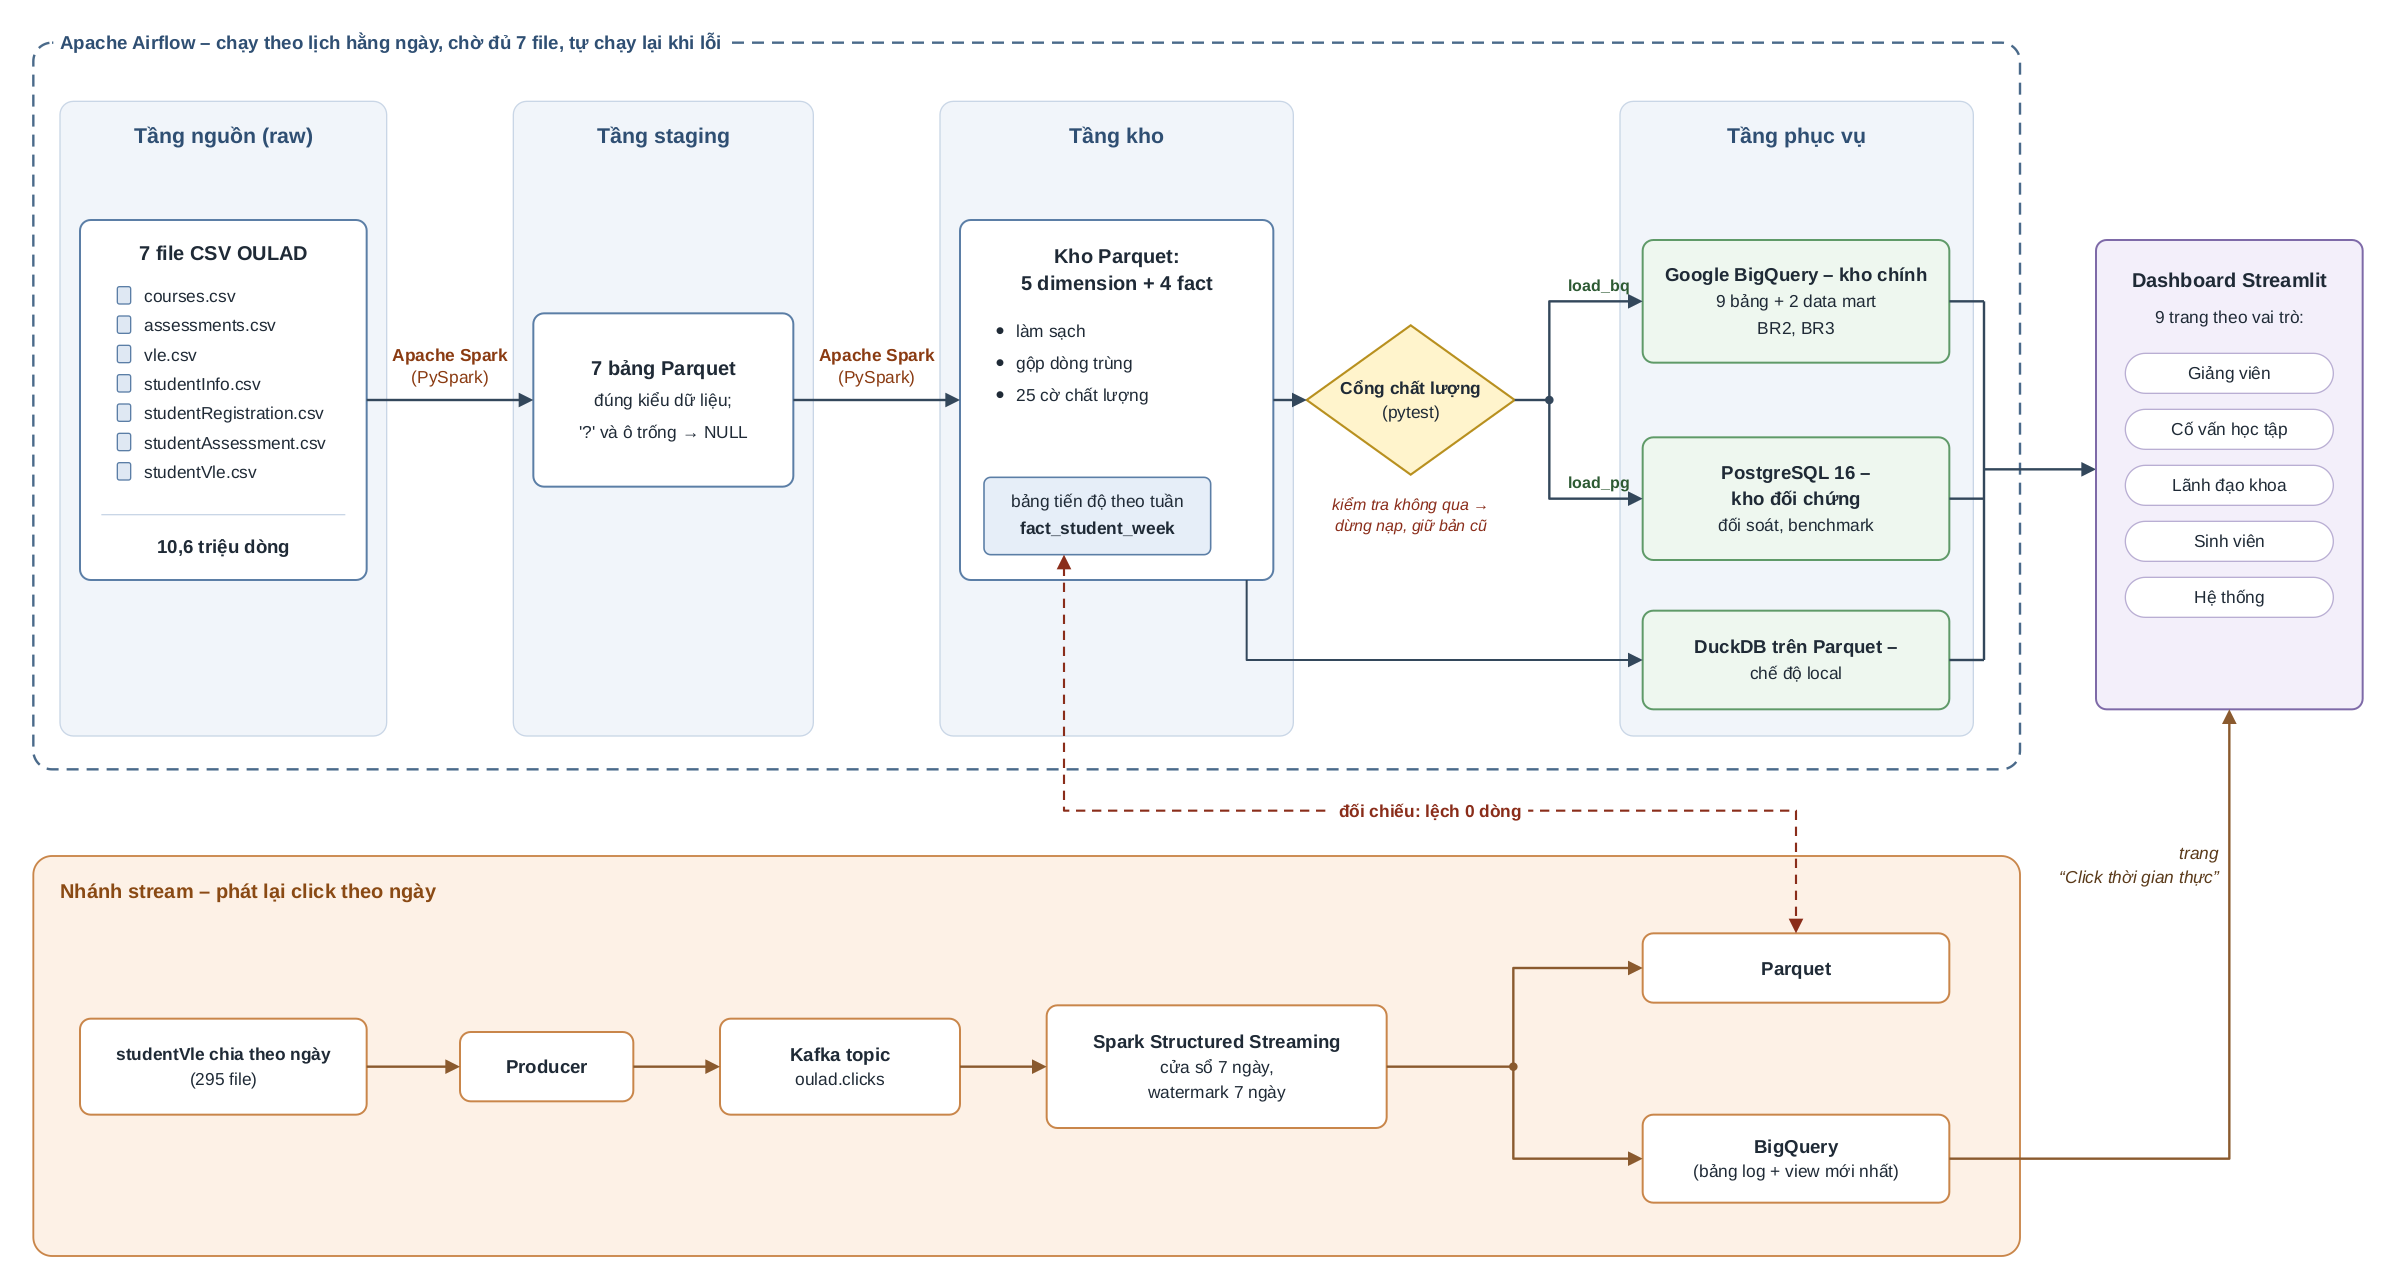
\includegraphics[width=\textwidth]{Images/Kien_truc.png}
\caption{Kiến trúc tổng thể của hệ thống}
\label{fig:kien-truc}
\end{figure}

% ------------------------------------------------------------
\subsection{Công nghệ sử dụng}
\label{sec:cong-nghe}
% Trước đây là chương riêng; gộp vào đây để báo cáo có 7 chương theo tiêu chí cấu trúc.

Hệ thống được xây dựng hoàn toàn bằng công cụ mã nguồn mở, cộng với BigQuery ở gói miễn
phí (Sandbox). Bảng~\ref{tab:cong-nghe} liệt kê các công nghệ theo thứ tự dữ liệu đi qua:
môi trường chạy, xử lý, lưu trữ, điều phối, rồi phục vụ người dùng. Toàn bộ hệ thống chạy
trong Docker, và phiên bản của mọi thư viện Python đều được khóa cố định, nên dựng lại ở
máy nào cũng ra cùng một môi trường.

\begin{table}[htbp]
\centering
\small
\begin{tabularx}{\textwidth}{|l|l|l|X|}
\hline
\textbf{Công nghệ} & \textbf{Phiên bản} & \textbf{Vai trò} & \textbf{Lý do lựa chọn} \\ \hline
Docker, Docker Compose & Compose v2 & Môi trường & Cả nhóm chạy cùng một môi trường trên Linux và Windows, không phải cài tay Java, Spark hay thư viện \\ \hline
Python & 3.11 & Ngôn ngữ chung & Spark, Airflow, Streamlit và thư viện BigQuery đều dùng được từ Python, nên cả nhóm chỉ cần một ngôn ngữ \\ \hline
Apache Spark (PySpark) & 3.5.3 & ETL batch & Xử lý phân tán; cùng một đoạn code chạy được trên một máy lẫn trên cụm \\ \hline
Apache Kafka & 3.8.1 & Hàng đợi sự kiện & Tách bên gửi click khỏi bên xử lý; Spark đọc theo offset và lưu offset vào checkpoint, nên dừng rồi chạy lại vẫn đọc tiếp đúng chỗ \\ \hline
Spark Structured Streaming & 3.5.3 & Xử lý stream & Cùng engine và cách viết với ETL batch; hỗ trợ cửa sổ theo thời gian sự kiện và watermark để giới hạn bộ nhớ \\ \hline
Apache Parquet & & Kho trung gian & Lưu theo cột, giữ kiểu dữ liệu, mọi engine phía sau đều đọc được \\ \hline
Google BigQuery & Sandbox & Kho chính & Kho dữ liệu đám mây không cần quản trị máy chủ, tính tiền theo lượng dữ liệu quét \\ \hline
PostgreSQL & 16 & Kho đối chứng & Đối soát kết quả với BigQuery; làm nền so sánh các cách tổ chức bảng \\ \hline
DuckDB & 1.5.6 & SQL tại máy & Chạy SQL thẳng trên file Parquet, dùng khi viết truy vấn và khi chạy test \\ \hline
Apache Airflow & 2.10.5 & Điều phối & Lập lịch, chờ dữ liệu đầu vào, kiểm tra chất lượng trước khi nạp, chạy lại khi lỗi \\ \hline
Streamlit, Plotly & 1.65.0, 6.9.0 & Dashboard & Viết giao diện bằng Python, không cần tầng backend riêng \\ \hline
pytest & 9.2.0 & Kiểm thử & Kiểm tra kho, đáp án nghiệp vụ, dashboard và pipeline \\ \hline
Make & & Chạy pipeline & Mỗi bước là một lệnh, dùng chung cho người chạy tay và cho Airflow \\ \hline
\end{tabularx}
\caption{Công nghệ sử dụng trong hệ thống}
\label{tab:cong-nghe}
\end{table}

\subsubsection{Lựa chọn engine xử lý}
File click lớn nhất có khoảng 10,6 triệu dòng. Lượng dữ liệu này một thư viện chạy trên
một máy như pandas vẫn xử lý được, nhưng nhóm chọn Spark vì ba lý do. Thứ nhất, khi dựng kho
lớn gấp 5 lần để đo hiệu năng, bảng click lên tới 42,3 triệu dòng. Thứ hai, Spark có cả
xử lý theo lô lẫn xử lý stream trên cùng một engine và cùng một cách viết. Thứ ba, xử lý
phân tán là một kiểu mẫu xử lý dữ liệu hiện đại mà môn học yêu cầu. Trong project, Spark
chạy ở chế độ local trên một máy; khi chuyển lên cụm thì code giữ nguyên, chỉ đổi cấu hình.

\subsubsection{Lựa chọn nơi lưu trữ}
Mỗi nơi lưu có một vai trò riêng. BigQuery là kho chính cho dashboard, vì không phải quản
trị máy chủ và lưu dữ liệu theo cột, nên truy vấn tổng hợp chỉ đọc những cột cần dùng. Gói
Sandbox miễn phí nhưng có giới hạn: tối đa 10 GB lưu trữ, bảng tự xóa sau 60 ngày, và không
cho dùng các lệnh sửa dữ liệu như \texttt{INSERT}, \texttt{UPDATE}. PostgreSQL lưu theo
dòng và có chỉ mục, nên được dùng làm kho đối chứng: cùng một truy vấn phải ra cùng kết quả
trên hai hệ thống có cách lưu khác nhau. DuckDB đọc thẳng file Parquet trên máy, giúp nhóm
viết và kiểm tra SQL nhanh mà không tốn hạn mức truy vấn của BigQuery. Vai trò của từng nơi
lưu trong kiến trúc được trình bày ở mục~\ref{sec:noi-luu}.

% ------------------------------------------------------------
\subsection{Các tầng dữ liệu}
\label{sec:cac-tang}

\textbf{Tầng nguồn (raw)} là 7 file CSV của OULAD, giữ nguyên như khi tải về. Pipeline chỉ
đọc tầng này, không bao giờ ghi đè, nên luôn có bản gốc để đối chiếu.

\textbf{Tầng staging} là bản sao của 7 file đó dưới dạng Parquet, mỗi file một bảng. Ở
bước này Spark chỉ đọc file theo kiểu dữ liệu khai báo sẵn và đổi các ký hiệu thiếu như
\texttt{"?"} hay ô trống thành giá trị rỗng (\texttt{NULL}); chưa có quy tắc nghiệp vụ nào
được áp dụng. Tách riêng tầng này giúp các bước sau làm việc trên dữ liệu đã đúng kiểu,
và khi kết quả sai thì biết ngay lỗi nằm ở dữ liệu nguồn hay ở phép biến đổi.

\textbf{Tầng kho} là kho dữ liệu theo dimensional model, gồm 5 bảng dimension và 4 bảng
fact (chương~\ref{sec:thiet-ke}), cũng lưu dưới dạng Parquet. Mọi bước làm sạch, gộp dòng
trùng, gắn cờ chất lượng và tính bảng tiến độ theo tuần đều diễn ra khi đi từ staging lên
tầng này. Bản kho trên Parquet là nguồn duy nhất cho mọi nơi lưu phía sau.

\textbf{Tầng phục vụ} là nơi người dùng và ứng dụng đọc dữ liệu: bản kho trên BigQuery và
PostgreSQL, cộng thêm hai bảng tổng hợp sẵn trên BigQuery cho BR2 và BR3. Hai bảng này gom
trước kết quả mà dashboard cần, nên mỗi lần mở trang không phải quét lại bảng click lớn.

% ------------------------------------------------------------
\subsection{Hệ lưu trữ và vai trò}
\label{sec:noi-luu}

Kho dữ liệu được hiện thực trên ba hệ lưu trữ, mỗi hệ đảm nhận một vai trò riêng. Lý do lựa
chọn từng công nghệ đã được trình bày ở mục~\ref{sec:cong-nghe};
Bảng~\ref{tab:noi-luu} tóm tắt dữ liệu lưu trữ và thành phần sử dụng của từng hệ.

\begin{table}[htbp]
\centering
\small
\begin{tabularx}{\textwidth}{|p{2.6cm}|p{2.9cm}|X|p{3.1cm}|}
\hline
\textbf{Hệ lưu trữ} & \textbf{Vai trò} & \textbf{Dữ liệu lưu trữ} & \textbf{Thành phần sử dụng} \\ \hline
Apache Parquet (truy vấn qua DuckDB) & Kho trung gian & Staging Area (7 bảng); Data Warehouse (5 dimension, 4 fact); bản mở rộng quy mô 5$\times$ & Pipeline ETL; phát triển và kiểm thử truy vấn; chế độ local của dashboard \\ \hline
Google BigQuery & Kho chính (Cloud Data Warehouse) & 9 bảng của Data Warehouse; 2 Data Marts; bản mở rộng quy mô 5$\times$; các mô hình dữ liệu thay thế phục vụ so sánh (3NF, wide table, nested) & BI Dashboard \\ \hline
PostgreSQL 16 & Kho đối chứng (Reference Warehouse) & 9 bảng của Data Warehouse; bản mở rộng quy mô 5$\times$; các mô hình dữ liệu thay thế phục vụ so sánh (3NF, wide table, JSONB) & Đối soát kết quả; đánh giá hiệu năng (benchmark) \\ \hline
\end{tabularx}
\caption{Các hệ lưu trữ và vai trò trong hệ thống}
\label{tab:noi-luu}
\end{table}

Vì có nhiều nơi lưu, hệ thống phải bảo đảm chúng không lệch nhau. Sau mỗi lần nạp, số dòng
của từng bảng trên BigQuery và PostgreSQL được so với số dòng trên Parquet. Ngoài ra, SQL
của 20 câu hỏi mẫu được viết theo cú pháp chung chạy được trên cả BigQuery, PostgreSQL và
DuckDB, và cả ba phải ra cùng đáp án. Nhờ vậy, khi một nơi cho kết quả khác, nhóm biết lỗi
nằm ở bước nạp vào nơi đó chứ không phải ở logic nghiệp vụ.

% ------------------------------------------------------------
\subsection{Luồng nạp batch}
\label{sec:luong-batch}

Luồng batch dựng lại toàn bộ kho từ 7 file CSV qua các bước theo thứ tự:
\begin{enumerate}
  \item \textbf{Staging}: đọc 7 file CSV, ghi 7 bảng Parquet.
  \item \textbf{Dimension}: làm sạch, dựng 5 bảng dimension và bảng fact đăng ký.
  \item \textbf{Fact}: dựng bảng fact click theo ngày và bảng fact nộp bài.
  \item \textbf{Bảng tiến độ theo tuần}: dựng ảnh chụp tiến độ của mỗi sinh viên theo tuần.
  \item \textbf{Nạp}: chép 9 bảng của kho lên BigQuery và PostgreSQL.
  \item \textbf{Kiểm thử}: chạy bộ kiểm thử trên kho vừa dựng.
\end{enumerate}

Mỗi bước ghi đè hoàn toàn kết quả cũ thay vì ghi thêm, nên chạy lại bao nhiêu lần cũng ra
cùng một kết quả, không sinh dòng trùng. Cả luồng chạy được bằng một lệnh và dừng ngay ở
bước lỗi đầu tiên. Nội dung và thời gian của từng bước được trình bày ở mục~\ref{sec:etl}.

% ------------------------------------------------------------
\subsection{Luồng stream}
\label{sec:kien-truc-stream}

OULAD là dữ liệu lịch sử, không có luồng sự kiện thật, nên nhánh stream phát lại click theo
từng ngày để mô phỏng dữ liệu đến dần. Nhánh này chạy song song với luồng batch và chỉ tính một
phần của kho: tổng click theo sinh viên, đợt học và tuần, tức các cột \texttt{clicks\_week},
\texttt{clicks\_cum} của bảng tiến độ theo tuần. Click của mỗi ngày được gửi vào Kafka, Spark
Structured Streaming đọc Kafka và cộng dồn theo tuần, rồi ghi kết quả ra Parquet và nạp lên
BigQuery sau mỗi lô nhỏ (micro-batch); trang dashboard đọc kết quả đó. Bản batch vẫn là nguồn
chuẩn: kết quả stream được đối chiếu với bảng tiến độ theo tuần của batch để chứng minh hai nhánh
cho cùng số liệu (mục~\ref{sec:stream}).

% ------------------------------------------------------------
\subsection{Điều phối}
\label{sec:dieu-phoi}

Luồng batch được Airflow điều phối. Airflow chạy các bước trên theo lịch hằng ngày, chờ đủ
7 file nguồn rồi mới bắt đầu, và tự chạy lại một bước khi bước đó lỗi. Điểm quan trọng nhất
là \textbf{cổng chất lượng}: sau khi dựng xong kho trên Parquet và trước khi nạp, Airflow
chạy các bài kiểm tra trên kho. Nếu có bài kiểm tra không qua, việc nạp bị dừng và
BigQuery, PostgreSQL vẫn giữ bản cũ, nên dashboard không bao giờ đọc phải dữ liệu sai. Hai
bước nạp BigQuery và PostgreSQL chạy song song vì không phụ thuộc nhau. Chi tiết cách hiện
thực ở mục~\ref{sec:airflow}.

% ------------------------------------------------------------
\subsection{Tầng phục vụ}
\label{sec:tang-phuc-vu}

Người dùng làm việc với hệ thống qua một dashboard viết bằng Streamlit, gồm 9 trang chia
theo nhóm người dùng: Chung, Giảng viên, Cố vấn học tập, Lãnh đạo khoa, Sinh viên và Hệ thống
(trang chất lượng dữ liệu, kết quả đo hiệu năng). Cả 9 trang đọc dữ liệu qua một lớp truy
vấn chung, không gọi thẳng vào nơi lưu. Lớp này chọn đọc từ BigQuery hay từ Parquet (qua
DuckDB) theo một biến cấu hình, nên cùng một dashboard chạy được trên đám mây lẫn trên máy
không có kết nối BigQuery. Kết quả truy vấn BigQuery được lưu tạm từ 1 đến 6 giờ tùy trang,
vì kho chỉ đổi khi nạp lại và mỗi lần truy vấn đều tính tiền theo lượng dữ liệu quét.
Mục~\ref{sec:dashboard} nêu cụ thể mỗi trang đọc những bảng nào của kho.

% ------------------------------------------------------------
\subsection{ETL và ELT}
\label{sec:etl-elt}

Trong ETL (Extract -- Transform -- Load), dữ liệu được biến đổi xong rồi mới nạp vào kho.
Trong ELT (Extract -- Load -- Transform), dữ liệu thô được nạp vào kho trước, rồi biến đổi
bằng SQL ngay trong kho. Hệ thống dùng cả hai. Phần chính là ETL: Spark làm sạch và dựng
toàn bộ dimension và fact trên Parquet, sau đó mới nạp lên BigQuery và PostgreSQL. Cách này
giữ logic biến đổi ở một chỗ duy nhất, nên mọi nơi lưu nhận cùng một kết quả. Phần nhỏ là
ELT: hai bảng tổng hợp sẵn cho BR2 và BR3 được tính bằng SQL ngay trên BigQuery từ các bảng
đã nạp, vì chúng chỉ phục vụ dashboard đọc từ BigQuery.
